\documentclass{article}
\usepackage[a4paper, margin=2.5cm]{geometry}
\usepackage{amsmath}
\usepackage{caption}
\usepackage{placeins}
\usepackage{graphicx}
\usepackage{subcaption}
\usepackage{setspace}
\usepackage{float}

%\usepackage[active,tightpage]{preview}
\usepackage{natbib}
\bibpunct{(}{)}{,}{a}{}{;} 
\usepackage{url}
\usepackage{nth}
\usepackage{authblk}
% for the d in integrals
\newcommand{\dd}{\; \mathrm{d}}
\newcommand{\tc}{\quad\quad\text{,}}
\newcommand{\tp}{\quad\quad\text{.}}
\defcitealias{HMD}{HMD}

\newcommand\ackn[1]{%
  \begingroup
  \renewcommand\thefootnote{}\footnote{#1}%
  \addtocounter{footnote}{-1}%
  \endgroup
}
\begin{document}

%\title{Macro patterns in the shape of aging}
\title{Flow decompositions in multistate Markov models}
\author[1]{Tim Riffe\thanks{riffe@demogr.mpg.de}}
\affil[1]{Max Planck Institute for Demographic Research}
\maketitle

\begin{abstract}
I demonstrate the application of standard decomposition techniques to decompose
differences between synthetic indices derived from age-stage Markov matrix
models into differences due to each stage transition. An example is given on the basis
of transition matrices from an analysis of working life expectancy in the
United States.
\end{abstract}

\section{Introduction}
I describe the application of a generic pseudo-continuous time decomposition
\citep{horiuchi2008} of differences between synthetic indices derived from two
sets of transition probabilities into differences from each each age-stage transition. Intuitively this means
we can assign how much of a difference is due to differences in each arrow in
the state-space diagram of the model in question. We demonstrate this
decomposition technique using published transition matrices from a recent study
of working life expectancy in the United States \citep{Dudel2017}.

\section{Method}
\subsection{Calculate the index, $\theta$ from exit probabilities}
Say we have a model with $s$ states and $\omega$ age classes, and manage to
produce matrix of transition probabilities, $\textbf{U}$, with ages nested
within block matrices of state transitions. This matrix will be square of
dimension $s\omega \times s\omega$, and each $\omega \times \omega$ block in
$\textbf{U}$ contains the transition probabilities from state $j$ to state $i$
in its subdiagonal. We'll follow the convention of \emph{from} states $j$ in
columns and \emph{to} states $i$ in rows. Now,
the main subdiagonal of $\textbf{U}$ contains the probabilities of staying in
one's state and advancing to the next age, often represented as
\emph{self} arrows in reduced state-space diagrams. 

Now say we calculate some quantity $\theta$ from $\textbf{U}$, that depends on
all its transition probabilities, such as an expected state occpancy (e.g. health
or employment). Define the function summarizing all the steps involved in
calculating $\theta$ from $\textbf{U}$:
\begin{equation}
 \theta = f^\theta(\textbf{U})
\end{equation}
Although expectancies and such are calculated on the
basis of \emph{living} transition probabilities, for purposes of decomposition
they are best treated as a function of \emph{exits} in general. By analogy, when
decomposing differences in life epectancy from the lifetable, we always
decompose with respect to death transitions and not age-specific survival
probabilities. The same rule applies to state occupancies with many potential
exits. If we wish to partition an expected state occupancy into contributions
from each of the various transitions, we therefore need to include death
transitions and exclude self-transitions from the decomposition. We therefore
require a function to convert a vector of all transfer probabilities implying
state exit into the matrix $\textbf{U}$. This is more a matter of program
organization that it is of mathematical notation. We know from the lifetable
that $p_x = 1 - q_x$. Translating this to the present situation, given a set of
exit probabilities, we can derive self-transition probabilities, $p_{s,s}$ in
much the same way:
\begin{equation}
 p_{s,s} = \left[1 - \sum p_{i,s} \right] \quad \text{for~} i \ne s
\end{equation}
Assume we have a vector of exit probabilities, $\textbf{p}^{(i \ne s)}$ then it
is possible to convert this into the required matrix $\textbf{U}$ via some steps
in a function $g^U$:
\begin{equation}
\textbf{U} = g^U\left(\textbf{p}^{(i \ne s)}\right)
\end{equation}
Then we can calculate our indicator from exit probabilities like so:
\begin{equation}
\theta = f^\theta\left(g^U\left(\textbf{p}^{(i \ne s)}\right)\right)
\end{equation}
Let's make notation easier and wrap that all in a function $\zeta$:
\begin{equation}
\label{eq:zeta}
\theta = \zeta\left(\textbf{p}^{(i \ne s)}\right)
\end{equation}
Now $\zeta$ is a function that is decomposable using generic decomposition
methods, such as the pseudo continuous method of \citet{horiuchi2008}, which
merits a brief summary.

\subsection{Summary of Horiuchi's decomposition method}
Given two vectors of equal structure and length $\textbf{p}^{1(i \ne s)}$ and
$\textbf{p}^{2(i \ne s)}$ (henceforth $\textbf{p}^1$ and $\textbf{p}^2$), which
may refer to two different populations or time points, we may calculate
$\theta^1$ and $\theta^2$ via \eqref{eq:zeta}.
The difference between $\theta^2$ and $\theta^1$, $\Delta^{(\theta)}$ can be
decomposed into contributions due to elementwise differences in $\textbf{p}^1$ and
$\textbf{p}^2$, $\Delta^{(p)}$ (also a vector). The method of
\citet{horiuchi2008} works by assuming a regular linear (though this is not necessary) change transforming $\textbf{p}^{1}$ into
$\textbf{p}^{2}$. Say we move from $\textbf{p}^1$ to $\textbf{p}^2$ in $n$
steps. In each step, each element moves $\Delta^{(p)} \frac{1}{n}$ of the respective difference. Within each step, there is therefore a new vector
composed of an intermediate set of values, $\textbf{p}^n$ from which $\theta$
may be recalculated. In each of the $n$ steps, we perturb the elements of
$\textbf{p}^n$ one at a time, pushing up the $i^{th}$ element
$\frac{\Delta^{(p)}[i]}{2n}$, calculating $\theta^{+i}$, then pushing the same
element down by the same amount and calculating $\theta^{-i}$. The difference between $\theta^{+i}$ and
$\theta^{-i}$ is taken as the contribution to $\theta^2-\theta^1$ from element
$i$ in step $n$. If there are $s\times\omega$ elements of
$\textbf{p}^{(n)}$, we recalculate $\theta$ a total of $n\times2\times
s\times\omega$ times. When complete, these contributions sum to
$\theta^2-\theta^1$ with a trivial error that depends mostly on $n$.
Typically, the contributions for each age and stage are summed over the $n$ ``time'' steps used in the procedure, producing a total of
$s \times \omega$ contributions that are the output that the researcher is
actually interested in. This vector of contributions can be aggregated in any
way to suit the needs of the researcher and facilitate interpretation. 

Even if $\zeta$ is simple, this procedure is computationally
intensive. The only parameter that can easily be changed is $n$, the number of
``time'' steps. \citet{horiuchi2008} recommend 20 as a practical number of
steps, and in my own experience there is little payoff for using an $n$ of 100.
In the following demonstration we'll opt for an $n$ of 10. Depending on the
size of the exercise at hand, it may be worth the researcher's time to efficiently program $\zeta$.

The researcher may of course swap out the Horiuchi method for a different
generic decomposition method, such as Blinder-Oaxaca decomposition
\citep{blinder1973wage, oaxaca1973male} or life table response experiments
\citep{caswell1989analysis}. I've opted for Horiuchi decomposition because it is
implemented in a generic form \texttt{R} in the package
\texttt{DecompHoriuchi}\footnote{\texttt{DecompHoriuchi} can be installed from
\texttt{github}: \url{https://github.com/timriffe/DecompHoriuchi}.}, which means
I only need to write a function that does \eqref{eq:zeta}.

\section{Application}
I apply this approach to a few of the transition matrices published
by \citet{Dudel2017} for ages 50+. Specifically, I decompose differences in
working life expectancy (WLE). The reduced (not showing
age) state space graph of this model is as drawn in Figure~\ref{fig:dudelstates}. Note that the elements of $\textbf{p}$ are all arrows leaving a given state not including self-arrows. This is transformed to $\textbf{U}$, which contains all
arrows including self-arrows and excluding arrows pointing to death. 

\begin{figure}[ht!]
\begin{center}
\caption{State space graph of \citet{Dudel2017}}
\label{fig:dudelstates}
\includegraphics[scale=.12]{Figures/StateSpace.jpg}
\end{center}
\end{figure}

We haphazardly select four matrices from which to make two comparisons: black
females in 2004 vs 2009, and high versus low-educated black females in
2009.\footnote{The requisite matrices come from the files
\texttt{Pmat\_b\_f\_2004.csv}, \texttt{Pmat\_b\_f\_2009.csv}, \texttt{Pmat\_b\_f\_edu0\_2009.csv}, and
\texttt{Pmat\_b\_f\_edu2\_2009.csv}, respectively. } Black females at age 50 had
a WLE of 10.1 in 2004, which dropped to 9.2 in 2009, for a difference of .9
years. This difference breaks down per Table~\ref{tab:A}
\FloatBarrier
% latex table generated in R 3.4.0 by xtable 1.8-2 package
% Thu Oct 12 14:37:54 2017
\begin{table}[ht]
\centering
\caption{Decomposition of .9 decrease in WLE from 2004-2009, black females.
``From'' states in columns, ``to'' states in rows.}
\label{tab:A}
\begin{tabular}{c|rrr}
 & W & I & R \\ 
  \hline
W &  & -0.51 & 0.05 \\ 
  I & -0.12 &  & 0.03 \\ 
  R & -0.20 & -0.01 &  \\ 
  D & -0.13 & -0.04 & 0.03 \\ 
   \hline
\end{tabular}
\end{table}

From this it is clear enough that the greatest driver of the drop in WLE was due
to decreased transitions from inactive to working states, as well as increased
exits from working into all other states. Further, it would appear that
retirement exits acted in small part to increase time spent working, either
directly by transitions to work, or indirectly by decreased mortality or increasing the pool
of inactive workers that then might transition into work. There are only nine
numbers in this table, so it can be interpreted directly. However, for models
with more states, or for many comparisons, it is better to move to visualization
to detect patterns. 

Table~\ref{tab:A} may be redrawn as Figure~\ref{fig:deca}, where each cell
represents a table element following the same ordering. Colored bars are
proportional to the values, but rescaled such that the maximum absolute
contribution is a 100\% filled box. Blue indicates negative contributions and
red indicates positive contributions. From this view it is easier to surmise
that the drop in transitions from inactive to working is roughly equal to all
increased flows out of employment combined. Such tables could in principle also
be composed in small multiples, in which case it would be advisable to have
equal y ranges between individual plots.

\begin{figure}[ht!]
\begin{center}
\caption{Visualization of Table~\ref{tab:A}. Red and blue indicate positive and
negative contributions, respectively. }
\label{fig:deca}
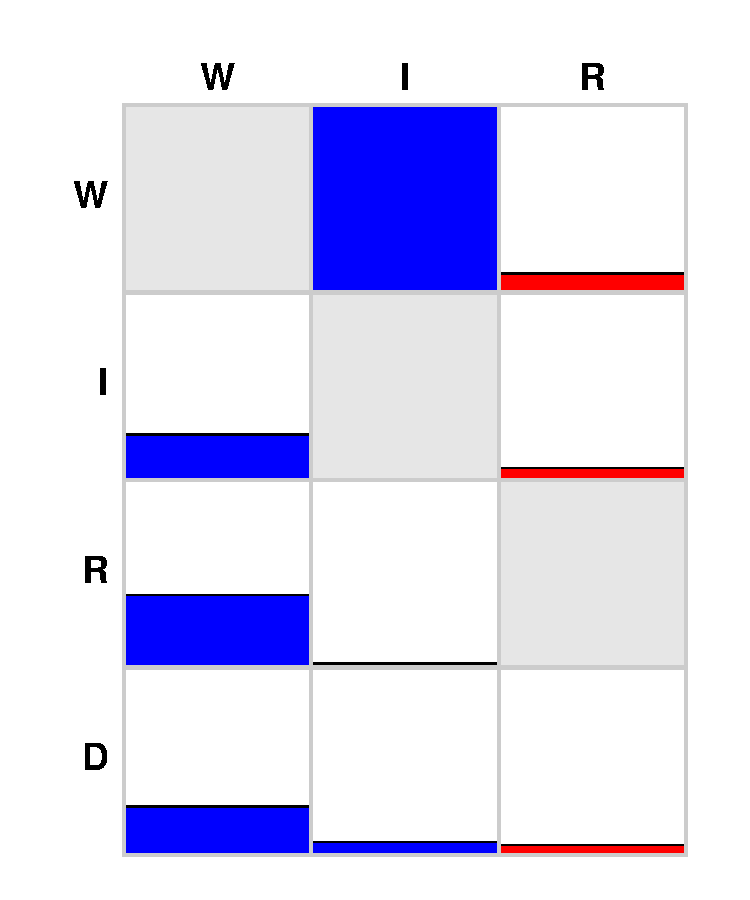
\includegraphics[scale=.5]{Figures/decA.pdf}
\end{center}
\end{figure}

For example, highly educated black females in 2009 had a WLE 2.26 years greater
than low educated bloack females. The largest single contribution to this
difference was due to mortality differentials of employed persons: 2.4 years.
Let's compare these decomposition results side-by-side with those of
Figure~\ref{fig:deca}, each proportionally scaled by the same amount.

\begin{figure}
\centering
\caption{Education differentials in WLE were greater in 2009 than the downward
change from 2004 to 2009 among US black females.}
\label{fig:deccompare}
\begin{subfigure}{.4\textwidth}
 \begin{center}
   \caption{Black females 2004 versus 2009 \\(0.9 year total gap)}
  \label{fig:deca2}
  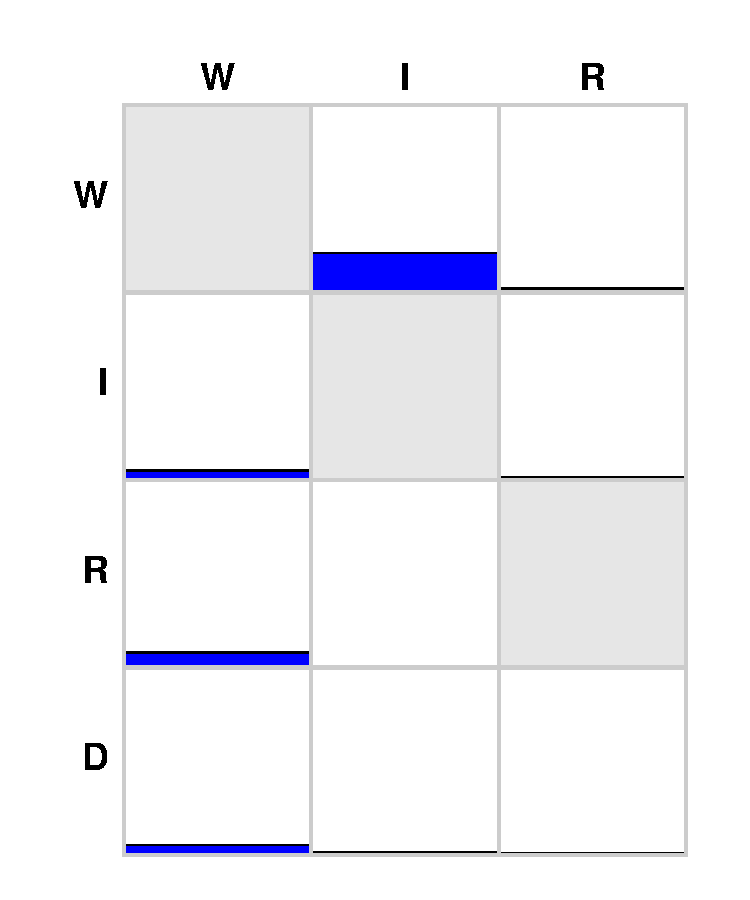
\includegraphics[width=.7\linewidth]{Figures/decA2.pdf}
 \end{center}
\end{subfigure}%
\begin{subfigure}{.4\textwidth}
  \centering
   \caption{High versus low educated, black females, 2009 \\(2.26 year total
   gap)}
  \label{fig:decb}
  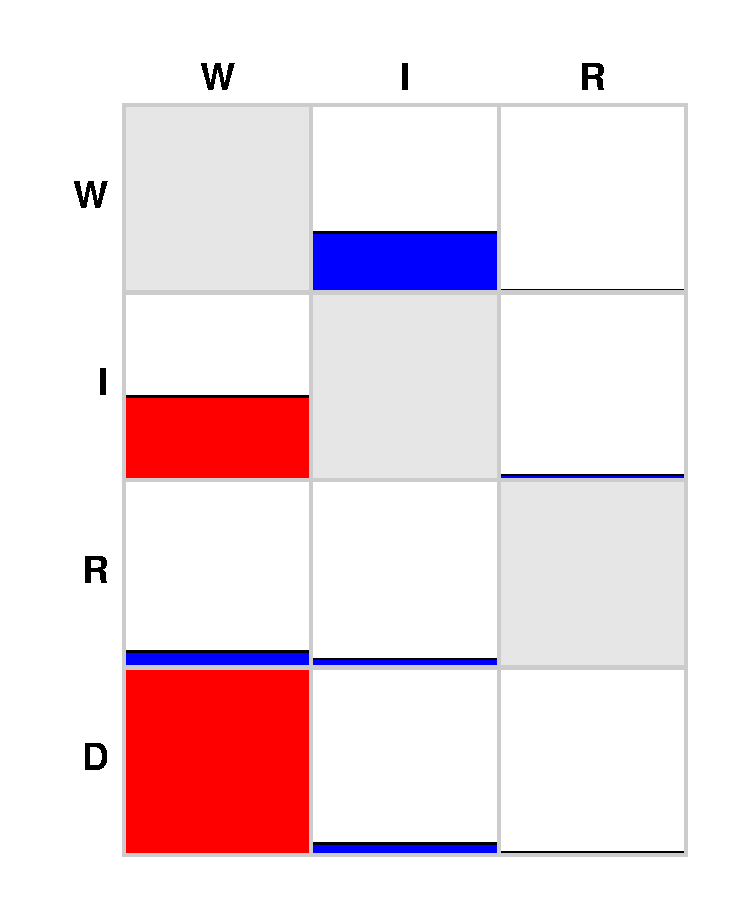
\includegraphics[width=.7\linewidth]{Figures/decB.pdf}
\end{subfigure}
\end{figure}

From Figure~\ref{fig:deca2} it is clear that the educational gradient in WLE was
greater in 2009 than the total loss in WLE from 2004 to 2009 among US black
females. Most of this differential was due to lower mortality and lower
transition rates from work to inactivity for highly educated black females. It's
worth mentioning that this positive gradient in 2009 was offset by greater
transitions from inactivity to employment for low-educated black females, and
that this contribution itself was roughly equal in magnitude to the total loss
in WLE from 2004 to 2009.
\FloatBarrier

\subsection{A word on weighting}
For this particular application, a vector $\pi$ is required to weight together
the initial populations of working, inactive, and retired persons at age 50,
where weights in higher ages assume a stationary propagation of the age 50
population.
\citet{Dudel2017} do not publish these values, so I assumed values of 0.7,
0.25, and 0.05 for all cases, which could be far from observed values. If true
weights are available, and if they differ between groups, then some differences
will indeed be due to weights themselves. Weights can therefore be included in
the vectors $\textbf{p}^1$ and $\textbf{p}^2$ and included in the decomposition
as well. That's optional, and it comes with its own bag of assumptions, such as
stationary generation of the weights from transitions in lower ages.

\section{Conclusions}
It is of course possible to not collapse age patterns: one could make stacked
bar charts typical of cause of death decompositions, but I think such
visualizations would be best used for analytic purposes. Instead my instinct is
that the decomposition results ought to enrich the discussion and interpretation
of results, such as SES gradients in expectancies. The same approach can be used
for incidence based models of health demography, for example to examine how much
of a change is due to changes in onset, recovery, or differential mortality.
This approach is advantegous also because it requires little deep thought or
programming to add onto an analysis. It has the potential to reveal things that
one might not have suspected at all, such as the huge influence of mortality on
educational gradients in WLE among US black females in 2009.\footnote{Maybe you
suspected this, I didn't} This note, along with \texttt{R} code used to generate
results, is acessible here:\\ \url{https://github.com/timriffe/ArrowDecomp}


\singlespacing
\bibliographystyle{plainnat}
  \bibliography{references} 

\end{document}
